\section{Intermezzo}
\label{sec:intermezzo}

\begin{frame}
	\frametitle{Intermezzo: Exams}
	\begin{center}
		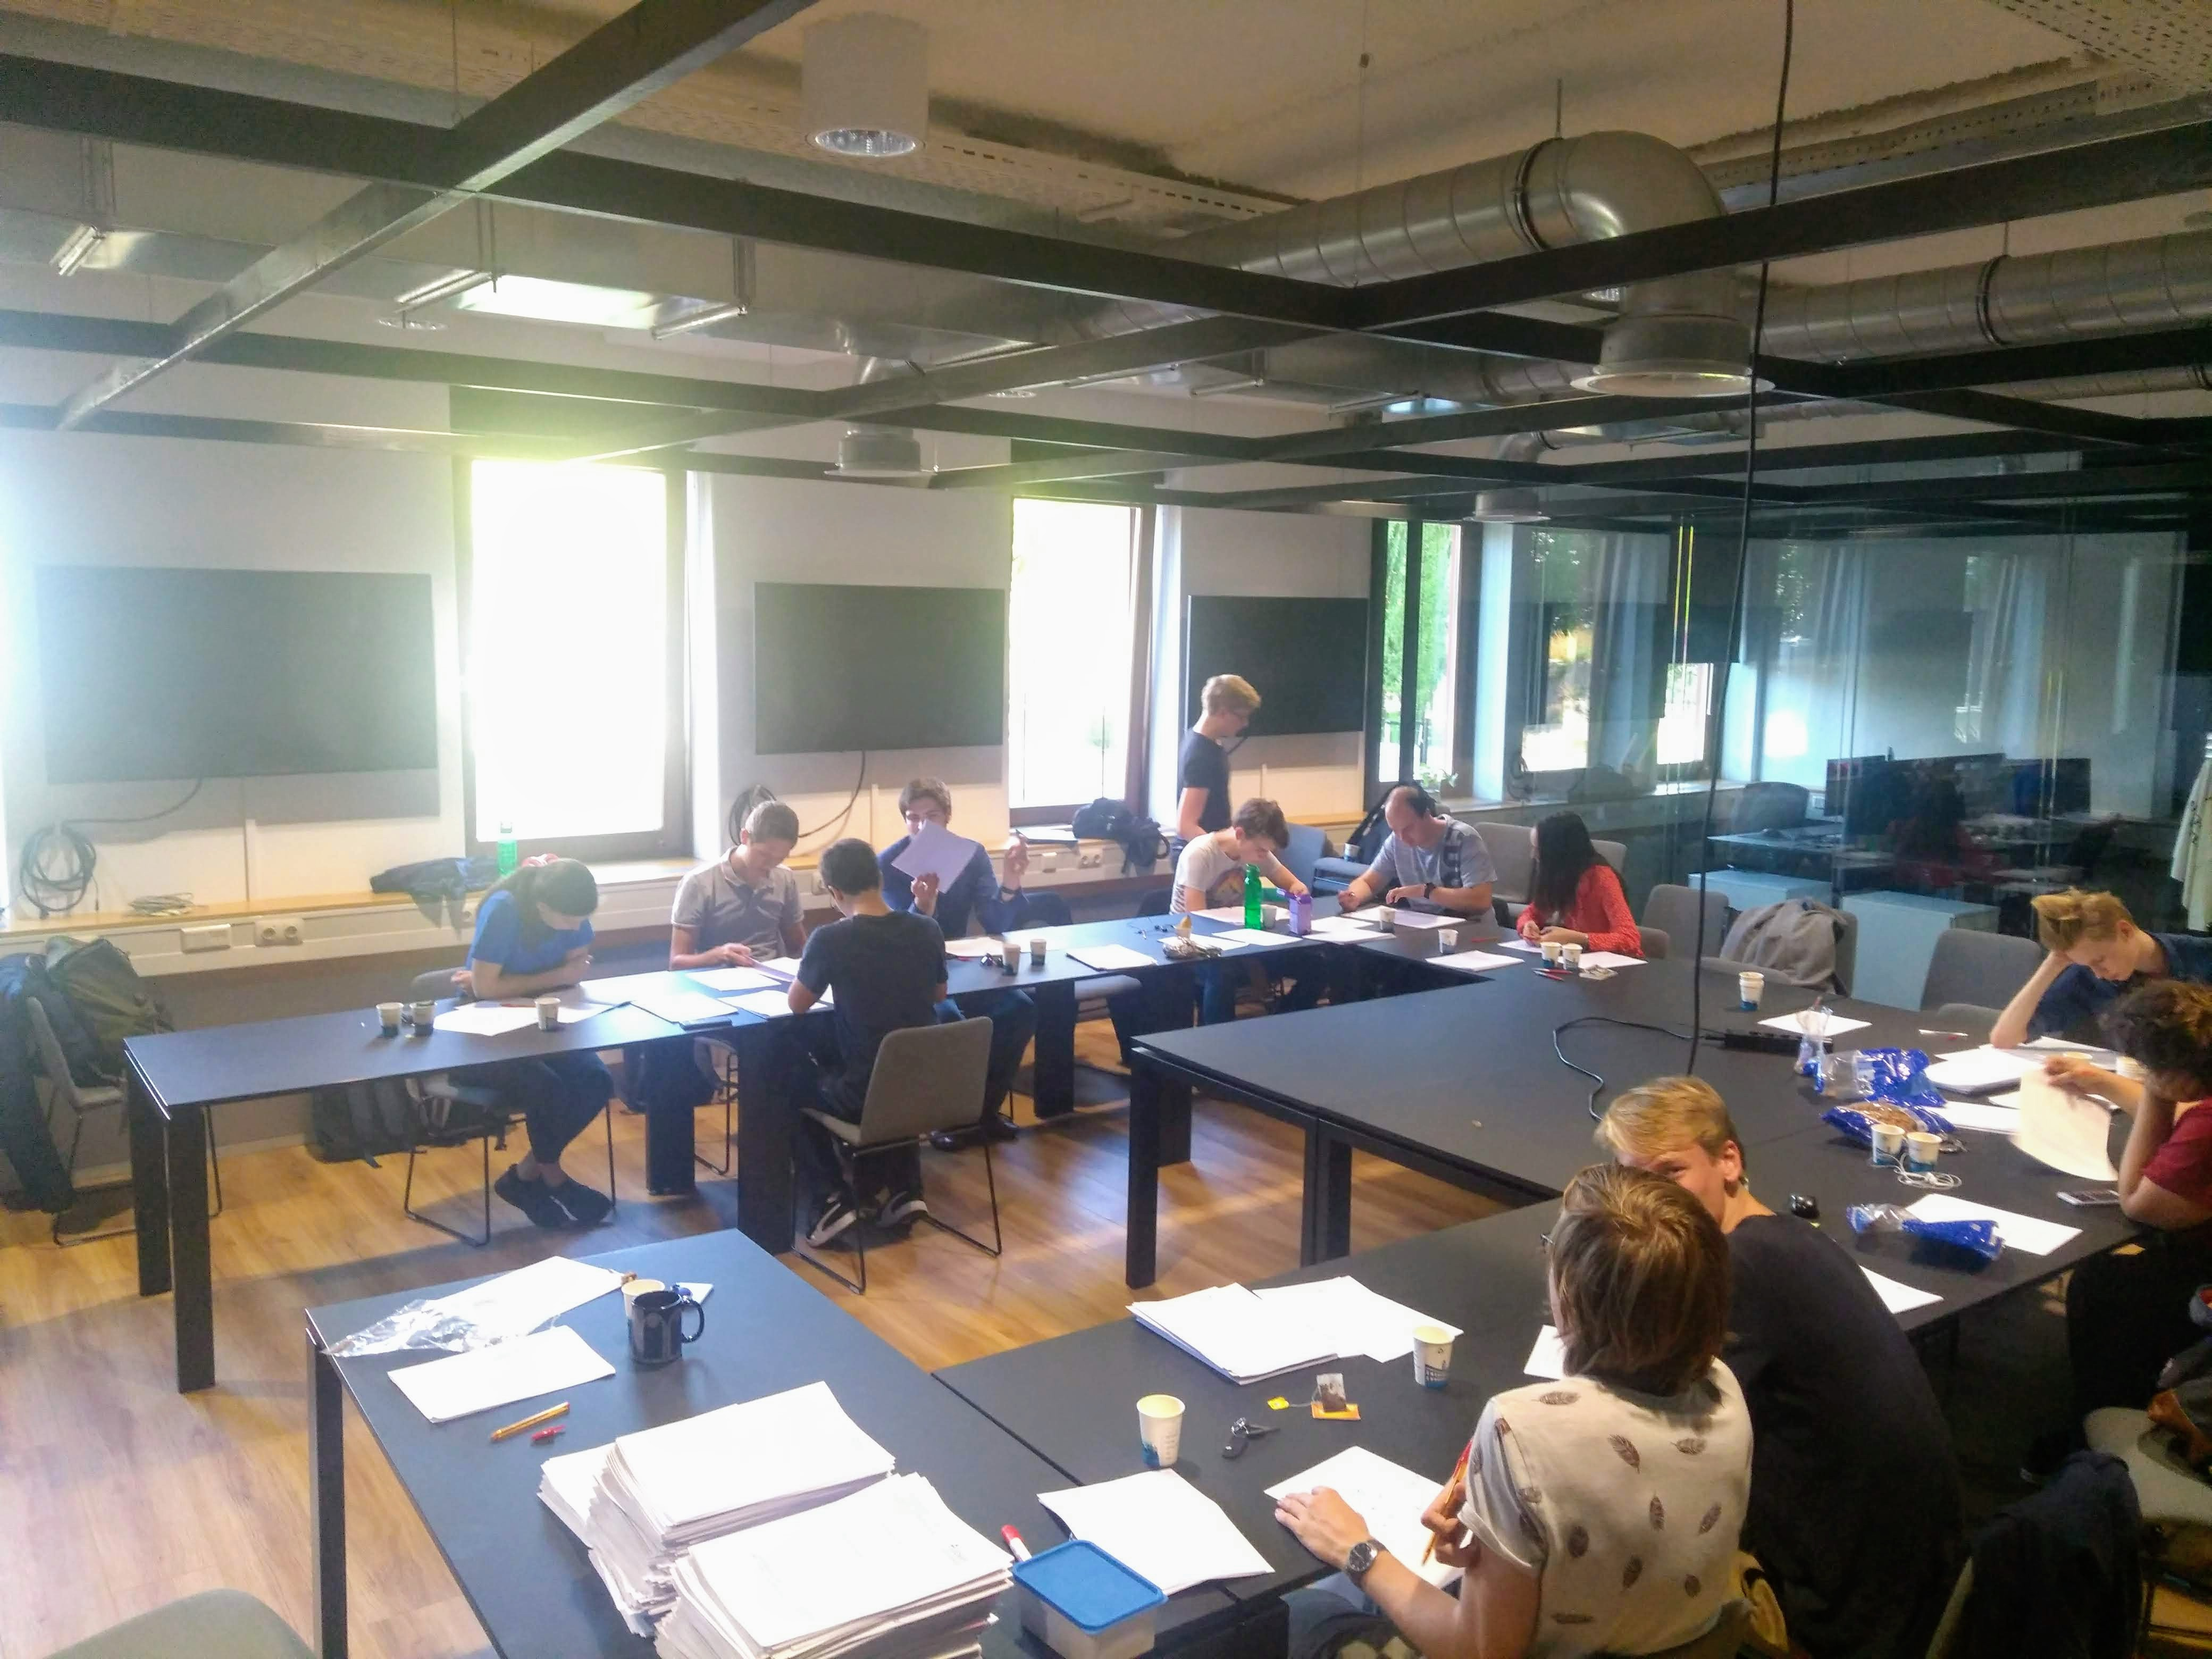
\includegraphics[width=0.6\textwidth]{figures/grading.jpg}\\
		\hspace*{15pt}\hbox{\scriptsize Image By:\thinspace{\itshape Stefan Hugtenburg}}
	\end{center}
\end{frame}

\begin{frame}
	\frametitle{The other type of tree}
	\framesubtitle{\url{https://science.howstuffworks.com/environmental/green-science/question16.htm}}
	\begin{itemize}
		\item We use a lot of paper, when it comes to exams\dots
			\pause
		\item Rough estimate of CSE first year, so far:
			\begin{itemize}
				\item 12 MC forms for 800 people
				\item 8 open question booklets for 800 people (2 sheets of paper each), assume everyone uses only one.
				\item 17 exams for 800 people, lets estimate that at 8 sheets each.
			\end{itemize}
			\pause
		\item	That's roughly 130-thousand sheets of paper.
			\pause
		\item Which is about 1.5 trees, according to howstuffworks.com
	\end{itemize}
\end{frame}

\begin{frame}
	\frametitle{Other interesting tree facts}
	\framesubtitle{\url{https://www.treesaregood.org/funfacts}}
	
	\begin{itemize}
		\item The oldest tree in the world is estimated at being 4765 years old.
			\pause
		\item The study of deteriming the age of a tree is called dendrochronology.
			\pause
		\item You are willing to pay more for goods and services if there are trees nearby! (slightly paraphrased)
			\pause
		\item Want to know more about where trees get their mass? Check this YouTube video:
			\url{https://www.youtu.be/2KZb2_vcNTg}
	\end{itemize}
\end{frame}

